\documentclass[../../main.tex]{subfiles}

% \usepackage{caption}
\captionsetup[table]{name=Tabla}

\begin{document}
\begin{frame}{Producción de gasolinas}{}

Una compañía de petróleos produce tres tipos de gosolinas: Súper, Normal y Euro. Se obtienen Por mezcla de tres calidades de crudos (A,B,C) que contienen tres componentes (1,2,3). La participación de estos componentes en la composición de cada crudo se muestra en la Tabla~\ref{tbl:composition} y las especificaciones de los tres tipos de gasolina en la Tabla~\ref{tbl:specification}.%


    \begin{columns}[t]
      \column{0.5\textwidth} \justifying     
      \begin{table}[!ht]
        \caption{\label{tbl:composition}Composición (\%) de cada crudo.}
    \centering
    \scalebox{0.90}{%
        \begin{tabular}{c|rrr}
    \toprule
          ~  & \multicolumn{3}{c}{Componentes} \\
          \midrule
      Crudos & 1 & 2 & 3 \\
      \midrule
        $A$ & 80 & 10 & 5 \\ 
        $B$ & 45 & 30 & 20 \\ 
      $C$ & 30 & 40 & 25 \\
      \bottomrule
        \end{tabular}%
      } % end scalebox
    \end{table}
    
    \column{0.5\textwidth}
    \begin{table}[!ht]
      \caption{\label{tbl:specification}Especificaciones (\%)}
    \centering
    \scalebox{0.90}{%
        \begin{tabular}{lrrr}
    \toprule
      ~  & 1 & 2 & 3 \\
      \midrule
        Súper & $\geq$ 60 & $\leq$ 25 & $\geq$ 10 \\ 
        Normal & $\geq$ 50 & $\leq$ 30 & $\leq$ 15 \\ 
      Euro & $\leq$ 40 & $\geq$ 35 & $\geq$ 20 \\
      \bottomrule
        \end{tabular}%
      } % scalebox
    \end{table}

    Ver Figura~\ref{fig:components}
    \end{columns}
 \end{frame}
  
\begin{frame}{Producción de gasolinas}
    Los costes por barril de crudos $A$, $B$ y $C$ son 650, 500 y 450 \$, respectívamente. El presupuesto diario de compra es de 50 millones \$; la disponibilidad diaria de crudos $B$ y $C$ se limita, respectivamente, a 3000 y 7000 barriles. Ciertos acuerdos obligan a comprar al menos 2500 barriles de $A$ por día. Las demandas de gasolina Súper y Normal son de 2000 y 2500 barriles diarios, que deben satisfacerse. La compañía desea maximizar la producción de gasolina Euro. Formular un modelo de programación lineal que dé respuesta al problema planteado por la compañía.%
  \end{frame}
    
  

\begin{frame}{Producción de gasolinas}
        \begin{figure}[h]
      \centering
        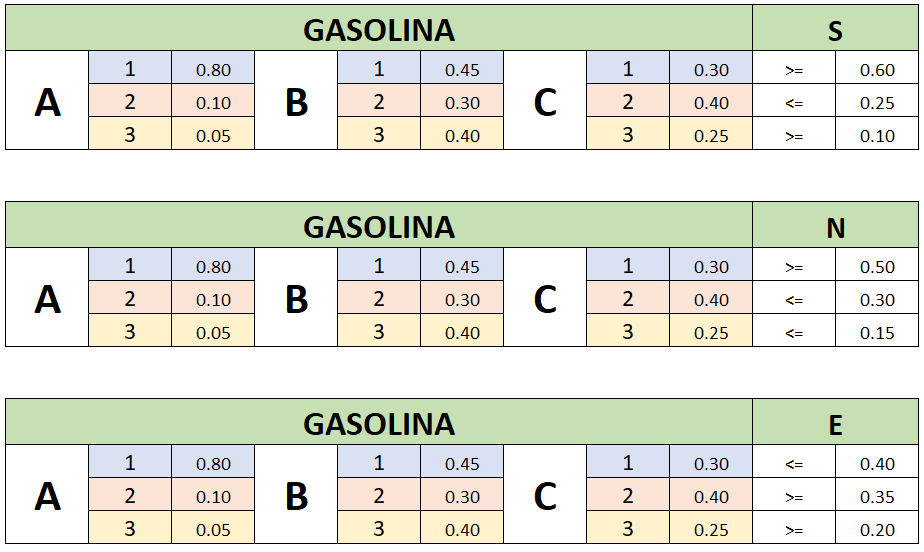
\includegraphics[scale=0.40]{03_gasoline-production.png}
      \caption{\label{fig:components}Composición de cada tipo de crudo}      
    \end{figure}
  \end{frame}
\end{document}
